\documentclass[a4paper,12pt]{article} % добавить leqno в [] для нумерации слева
\usepackage[a4paper,top=1.3cm,bottom=2cm,left=1.5cm,right=1.5cm,marginparwidth=0.75cm]{geometry}
%%% Работа с русским языком
\usepackage{cmap}					% поиск в PDF
\usepackage{mathtext} 				% русские буквы в фомулах
\usepackage[T2A]{fontenc}			% кодировка
\usepackage[utf8]{inputenc}			% кодировка исходного текста
\usepackage[english,russian]{babel}	% локализация и переносы

\usepackage{multirow}
\usepackage{graphicx}
\usepackage{mathtools}
\usepackage{wrapfig}
\usepackage{tabularx}
\usepackage{amssymb}
\usepackage{hyperref}
\usepackage[rgb]{xcolor}
\hypersetup{colorlinks=true,urlcolor=blue}
%% Шрифты
\usepackage{euscript}	 % Шрифт Евклид
\usepackage{amsmath}
\usepackage{mathtools}
%%% Заголовок
\author{Lokhmatov Arseniy}
\title{Лабораторная работа по общей физике}

\date{\today}
\begin{document}
\begin{titlepage}
    \newpage
    \begin{center}
    {\large МОСКОВСКИЙ ФИЗИКО-ТЕХНИЧЕСКИЙ ИНСТИТУТ (НАЦИОНАЛЬНЫЙ ИССЛЕДОВАТЕЛЬСКИЙ УНИВЕРСИТЕТ)}
    \vspace{1cm}

    {\largeФизтех-школа аэрокосмических технологий}
    \vspace{6em}
    \end{center}
    
    \vspace{1.2em}

    \begin{center}
    %\textsc{\textbf{}}
    \Large Лабораторная работа №4.4.2 \\
    Изучение фазовой решётки с помощью гониометра
    \linebreak
    \end{center}
    
    \vspace{11em}
    
    \begin{flushright}
                       {\large Работу выполнили\\
                       Лохматов Арсений Игоревич\\
                       Козярский Алексей Сергеевич\\
                       Б03-303 }
    \end{flushright}

    \vspace{\fill}

    \begin{center}
        
\includegraphics[width=0.2\linewidth]{dasr.png}
    \end{center}

    \begin{center}
    Долгопрудный, 2025
    \end{center}

    \end{titlepage}

\section{Теоретическая часть}


\paragraph{Цель работы: } ознакомиться с работой гониометра и определить спектральные характеристики фазовой решётки (эшелета).

\paragraph{В работе используются: } ртутная лампа, гониометр, фазовая дифракционная решётка, плоскопараллельная стеклянная пластинка, призменный уголковый отражатель, щель с микрометрическим винтом.

В современных спектральных приборах широко используются отражательные решётки с треугольным профилем штриха, так как они способны концентрировать дифрагированное излучение (до $70–80 \%$ мощности падающего излучения) в определённом (не нулевом) порядке. Отражательная решётка с треугольным профилем штриха (рисунок $\ref{img1}$), в которой угол $\Omega$ между рабочей гранью и плоскостью решётки (угол скоса) не превышает $20^\circ$, называется эшелетом. Рабочий порядок спектра, в котором концентрируется излучение, зависит от угла скоса и периода решётки и обычно невелик: $m\lesssim10$. Число штрихов на миллиметр $n=1200 – 0,3\text{ }\frac{\text{штр}}{\text{мм}}$.

\begin{figure}[h]
    \begin{center}
        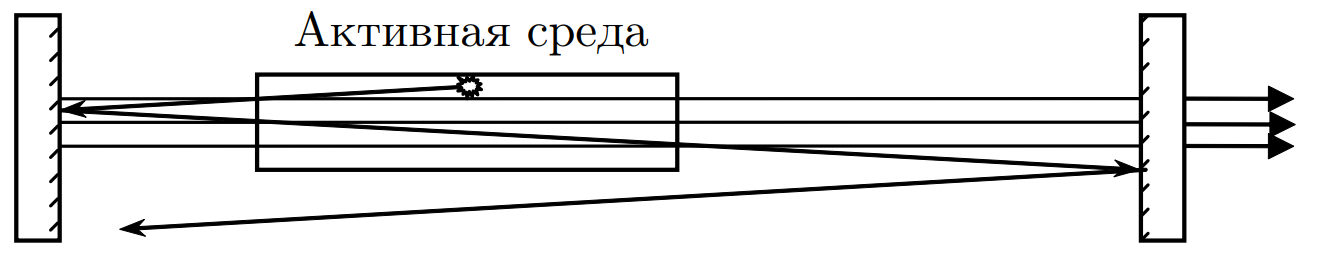
\includegraphics[width=11cm]{image1.png}
    \end{center}
    \caption{Распределение интенсивности в спектре эшелета}
    \label{img1}
\end{figure}

Если угол скоса $\Omega$ лежит в пределах $20 - 60^\circ$, решётка носит название эшелле. Рабочий порядок в такой решётке $m=5 - 500$, а число штрихов $n=10-100\text{ }\frac{\text{штр}}{\text{мм}}$. Теория отражательной решётки во многом сходна с теорией прозрачной (амплитудной) решётки. Пусть на решётку падает плоская монохроматическая волна ($\lambda$) под углом $\psi$, который отсчитывается от нормали $N_{\text{пл}}$ к плоскости решётки (рисунок $\ref{img1}$). Нас интересует распределение интенсивности волны, отражённой от решётки, в точке наблюдения, удалённой на бесконечность (в фокальной плоскости объектива зрительной трубы). На рисунке пунктирная кривая показывает распределение интенсивности $I_1(\varphi)$ света, дифрагировавшего на одной грани решётки, в зависимости от угла наблюдения $\varphi$. Все минимумы этой функции эквидистантны, боковые максимумы существенно меньше центрального. Угол, под которым наблюдается максимум интенсивности функции $I_1(\varphi)$, соответствует зеркальному отражению падающего луча от грани и называется углом блеска $\varphi_{\text{б}}$. Поскольку угол между нормалью к плоскости решётки $N_{\text{пл}}$ и нормалью к грани $N_{\text{гр}}$ равен углу скоса
$\Omega$, ясно, что угол блеска

\[ \varphi_{\text{б}}=\psi+2\Omega. \]

Суммарная амплитуда поля в бесконечно удалённой точке определяется, согласно принципу Гюйгенса–Френеля, суперпозицией волн, приходящих от различных граней решётки. На рисунке $\ref{img1}$ сплошная кривая показывает зависимость суммарной интенсивности света $I(\varphi)$ от угла наблюдения. Распределение $I(\varphi)$ имеет ряд резких максимумов.

Амплитуда поля в точке наблюдения максимальна, когда волны, приходящие от всех граней, оказываются в фазе. При этом разность хода $\Delta$ двух лучей $A'A$ и $B'B$, отражённых от соседних граней, кратна $\lambda$. Как видно из рисунка $\ref{img1}$, эта разность хода 

\[ \Delta=AC-BD=d(sin{\varphi_m}-sin{\psi})=m\lambda, \]

где $d$ — период решётки, $\varphi_m$ — угол, под которым наблюдается максимум, $m$ — порядок спектра. Будем считать углы положительными, если они отсчитываются против часовой стрелки от нормали $N_{\text{пл}}$, и отрицательными, если наоборот. С учётом принятого правила знаков условие дифракционного максимума для отражательной решётки примет вид

\[ d(sin{\varphi_m+sin{\psi})=m\lambda.} \]

На рисунке $\ref{img1}$ угол $\psi<0$, угол $\varphi_m>0$, порядок спектра положителен для максимумов, лежащих правее нулевого, если смотреть навстречу дифрагировавшим лучам. Из формулы следует, что $m=0$ при $\varphi_0 = -{\psi}$.

Изменяя угол падения света на эшелет, можно добиться того, чтобы угол блеска совпал с углом дифракции спектра одного из порядков. Ясно, что именно в этом порядке спектр будет наиболее ярким, так как он возникает при интерференции лучей, испытавших зеркальное отражение от рабочих граней решётки. Этот порядок спектра $m_p$ принято называть рабочим.

Чтобы устранить произвол в выборе угла падения света при определении рабочего порядка, принято считать, что решётка должна работать в автоколлимационном режиме, когда падающий луч параллелен отражённому. Для этого необходимо, чтобы свет падал перпендикулярно рабочей грани решётки, то есть $\psi=\varphi_m=\varphi_{\text{б}}=\Omega$. В этом случае условие принимает вид

\[ 2d\sin{\Omega}=m_p\lambda_p. \]

Если известна рабочая длина волны $\lambda_{p}$, вблизи которой локализован исследуемый спектр, выбраны шаг решётки $d$ и рабочий порядок спектра $m_{p}$, удобные для последующих измерений, то соотношение выше определяет угол скоса рабочей грани, который нужно реализовать при изготовлении эшелета. В этом случае исследуемый спектр будет наиболее ярким при работе в автоколлимационном режиме; в техническом паспорте эшелета указаны соответствующие значения $m_{p}$ и $\lambda_{p}$.

На рисунке $\ref{img1}$ приведена примерная зависимость интенсивности света от угла наблюдения для эшелета, предназначенного для работы в первом порядке. Наш эшелет отражает в спектр первого порядк а до $60\%$ мощности падающего излучения. Напомним, что спектр обычной амплитудной решётки наиболее интенсивен в нулевом порядке, где дисперсия $D=0$. Кроме того, в амплитудной решётке неизбежны значительные потери света, связанные с его поглощением непрозрачными участками решётки, размер которых существенно больше размера прозрачных участков.

Легко проверить, что разрешающая способность $R$ и дисперсионная область $G$ для эшелета вычисляются так же, как для амплитудной решётки. Для оценки угловой полуширины $\delta\varphi_{m}$ спектрального максимума воспользуемся методом векторных диаграмм. Амплитуду поля, пришедшего в бесконечно удалённую точку от граней решётки, будем изображать векторами $E_{n}$, где $n$ изменяется от единицы до $N$ ($N$ -- число отражающих граней). Длины векторов одинаковы для каждой грани, а угол $\theta$ между двумя соседними векторами зависит от разности хода: $\theta=2\pi\Delta/\lambda$.

\begin{figure}[h]
    \begin{center}
        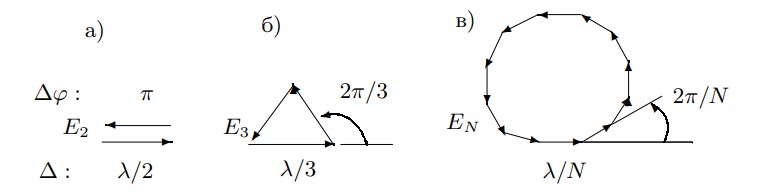
\includegraphics[width=14cm]{image2.png}
    \end{center}
    \caption{Векторные диаграммы}
    \label{img2}
\end{figure}

Как известно, две волны, пришедшие в точку наблюдения, погасят друг друга при разности хода между ними $\Delta=\lambda/2$ (рисунок $\ref{img2}$а). Следовательно, минимумы функции $I(\varphi)$ при дифракции на двух щелях лежат посредине между главными максимумами. При сложении трёх волн они погасят друг друга при выполнении условия $\Delta=\lambda/3$ (рисунок $\ref{img2}$б). При этом минимумы несколько приблизятся к максимумам, а в промежутке между минимумами появится небольшой дополнительный максимум. Очевидно, что при сложении волн, отражённых от $N$ щелей, суммарная амплитуда будет равна нулю, если разность хода между соседними векторами составляет $\lambda/N$ (рисунок $\ref{img2}$в). Таким образом, направление на минимум, ближайший к максимуму любого порядка, определяется условием

\[ d[\sin{(\varphi_m+\delta\varphi)}+\sin{\psi}]=m\lambda+\frac{\lambda}{N}. \]

Для малой полуширины максимума получим

\[ \delta\varphi=\frac{\lambda}{Nd\cos{\varphi_m}}. \]

Зависимость дисперсии $D$ от параметров эшелета можно найти, дифференцируя обе части выражения выше:

\[ D=\frac{m}{d\cos{\varphi_m}}=\frac{m}{\sqrt{d^2-(m\lambda-d\sin{\psi})^2}}. \]

Дисперсия растёт с увеличением порядка спектра и угла падения.

\newpage

\section{Практическая часть}

\subsection{Настройка гониометра}

Провели юстировку гониометра и установили начало отсчёта, руководствуясь правилами, изложенными в техническом описании (ТО).

\begin{figure}[h]
\begin{center}
\begin{minipage}[h]{0.4\linewidth}
    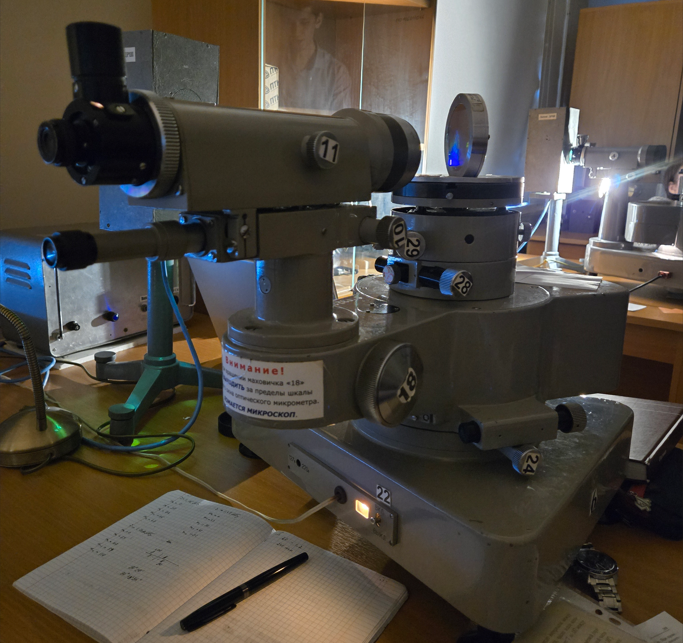
\includegraphics[width=1\linewidth]{goniometer.PNG}
    \caption{Гониометр} %% подпись к рисунку
    \label{ris:experimoriginal} %% метка рисунка для ссылки на него
\end{minipage}
\hfill
\begin{minipage}[h]{0.4\linewidth}
    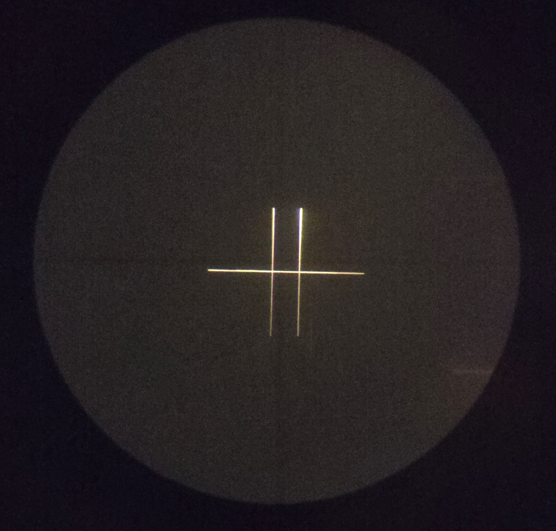
\includegraphics[width=1\linewidth]{cross.PNG}
    \caption{Юстировочный крест}
    \label{ris:experimcoded}
\end{minipage}
\vfill
\begin{minipage}[h]{0.4\linewidth}
    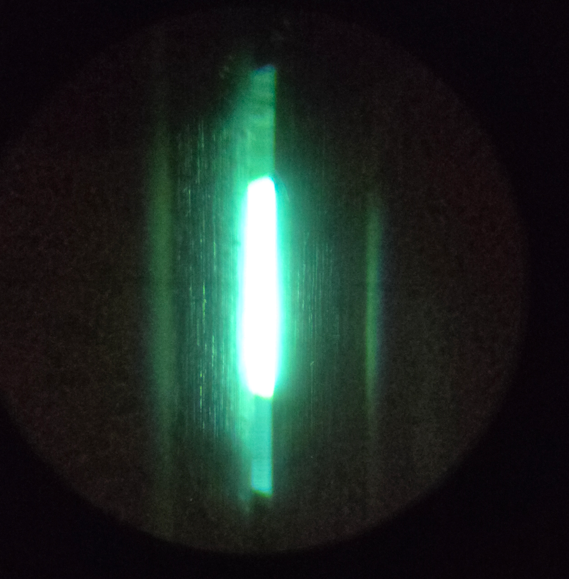
\includegraphics[width=1\linewidth]{slit.PNG}
    \caption{Изображение щели}
    \label{ris:experimcoded}
\end{minipage}
\hfill
\begin{minipage}[h]{0.4\linewidth}
    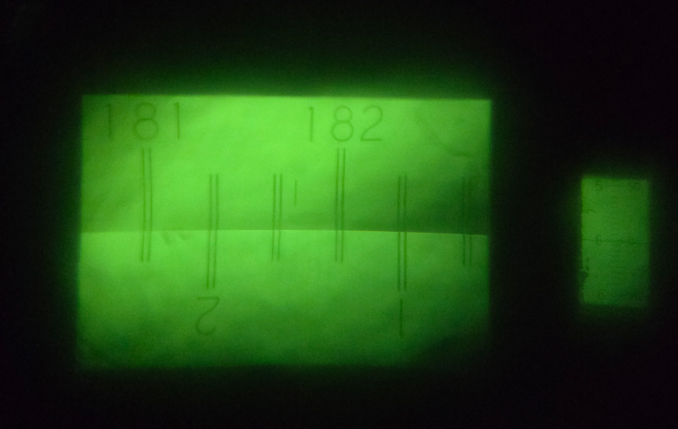
\includegraphics[width=1\linewidth]{scale.PNG}
    \caption{Отсчетная шкала гониометра}
    \label{ris:experimcoded}
\end{minipage}
\end{center}
\end{figure}

\subsection{Установка эшелета}


Необходимость дополнительной настройки столика с эшелетом связана с тем, что плоскость эшелета может быть не перпендикулярна его основанию. 

\begin{enumerate}
    \item Поставили эшелет на столик настроенного гониометра перпендикулярно одному из винтов $8$ и параллельно другому.
    \item Установив начальное положение трубы (против коллиматора) на $180^{\circ}$, поверните трубу на $120^{\circ}$ влево, так как при изучении эшелета убедились в том, что рабочий порядок эшелета положительный.

    Вращая только верхнюю часть столика (винт $26$ закреплён, чтобы не сбилась настройка нуля), нашли ахроматическое (белое) изображение щели, отражённой от эшелета. При этом угол падения света на плоскость эшелета $\psi$ составляет $(180^{\circ}-120^{\circ})/2=30^{\circ}$.
    \item Винтом $8$, перпендикулярным плоскости эшелета, установили короткое изображение на щелина центр поля зрения. Отводя алидаду в сторону от коллиматора, нашли в трубе спектр самого дальнего порядка и вторым винтом $8$ (параллельным плоскости эшелета) снова установили короткое изображение щели на центр.
    \item Вернулись к ахроматическому отражению и проверили результат. Так, методом последовательных приближений добились того, чтобы при повороте трубы изображение щели и спектр уходили не больше, че на треть радиуса поля зрения.
    \item Закончив настройку, подобрали ширину входной щели так, чтобы хорошо разрешались линии жёлтого дублета (ширина изображения щели чуть больше промежутка между линиями двойного штриха).
    Установили высоту щели, удобную для измерений.
\end{enumerate}

\subsection{Исследование спектра ртутной лампы}

\begin{enumerate}
    \item Для угла падения света на эшелет $\psi=30^{\circ}$ измерили угловые координаты спектральных линий ртути в рабочем порядке. Результаты представлены в таблице $\ref{tab1}$.

    \item Для оценки разрешающей способности эшелета оценили на глаз, во сколько раз расстояние между линиями дублета больше полуширины одной линии: $\sim12$. В описании к работе сказано, что расстояние между линиями можно принять за $\Delta\lambda=20\text{ А}$. Соответственно, ширина одной линии равна $\delta\lambda=\frac{20}{12}=1.67\text{ А}$. Тогда разрешающая способность эшелета при условии, что длина волны жёлтого света составляет $\lambda=5800\text{ А}$ находится по формуле:
    
    \[ R = \frac{\lambda}{\delta\lambda} = \frac{5800}{1.67} = 3473. \]
    
\end{enumerate}

 \begin{table}[h]
    \centering
    \begin{tabular}{|c|c|c|}
    \hline
    $ $ & $\varphi$ & $m_{\text{порядок}}$ \\ \hline
        \text{син.} & $60^{\circ}19'19''$ & -1 \\ \hline
        \text{фиол.} & $64^{\circ}39'19''$ & -1 \\ \hline
        \text{фиол.} & $64^{\circ}18'53''$ & -1 \\ \hline
        \text{щель} & $90^{\circ}16'57''$ & 0 \\ \hline
        \text{фиол.} & $107^{\circ}34'8''$ & 1 \\ \hline
        \text{фиол.} & $107^{\circ}42'25''$ & 1 \\ \hline
        \text{син.} & $108^{\circ}46'26''$ & 1 \\ \hline
        \text{син.-зел.} & $111^{\circ}14'4''$ & 1 \\ \hline
        \text{син.-зел.} & $111^{\circ}0'51''$ & 1 \\ \hline
        \text{зел.} & $113^{\circ}19'32''$ & 1 \\ \hline
        \text{жёлт.} & $114^{\circ}12'41''$ & 1 \\ \hline
        \text{жёлт.} & $114^{\circ}17'4''$ & 1 \\ \hline
        \text{крас.} & $116^{\circ}14'18''$ & 1 \\ \hline
        \text{жёлт.} & $134^{\circ}31'13''$ & 2 \\ \hline
        \text{жёлт.} & $134^{\circ}40'5''$ & 2 \\ \hline
    \end{tabular}
\caption{Положение спектральных полос ртутной лампы при угле падения лучей 45 градусов}
\label{tab1}
\end{table}

\newpage

\begin{figure}
    \centering
    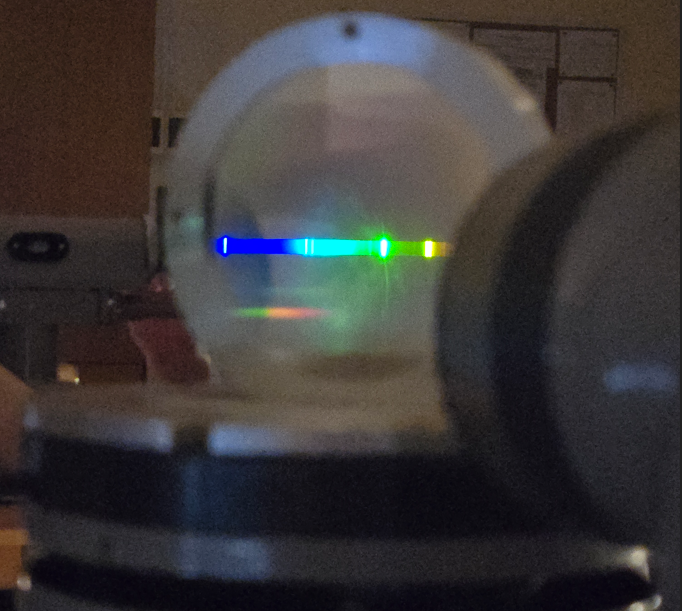
\includegraphics[width=0.5\linewidth]{spectrum.PNG}
    \caption{Наблюдаемый на эшелетте спектр}
    \label{fig:enter-label}
\end{figure}


\subsection{Зависимость дисперсии от угла падения в разных порядках}

\begin{enumerate}
    \item Для углов падения света на эшелет $\psi=30^{\circ}, 45^{\circ}, 60^{\circ}$ измерили координаты каждой из жёлтых линий дублета во всех наблюдаемых порядках, положительных и отрицательных. Заметили, при увеличении угла падения появляются спектры дальних отрицательных порядков. Результаты измерений представлены в таблице $\ref{tab2}$.
\end{enumerate}

\begin{table}[h]
    \centering
    \begin{tabular}{|c|c|c|}
    \hline
        \multicolumn{3}{|c|}{$\varphi=45^{\circ}$} \\ \hline
    \hline
    $ $ & $\varphi$ & $m_{\text{порядок}}$ \\ \hline
        \text{щель} & $90^{\circ}16'57''$ & 0 \\ \hline
        \text{жёлт.} & $114^{\circ}12'41''$ & 1 \\ \hline
        \text{жёлт.} & $114^{\circ}17'4''$ & 1 \\ \hline
        \text{жёлт.} & $134^{\circ}31'13''$ & 2 \\ \hline
        \text{жёлт.} & $134^{\circ}40'5''$ & 2 \\ \hline
    \end{tabular}
    \begin{tabular}{|c|c|c|}
    \hline
        \multicolumn{3}{|c|}{$\varphi=60^{\circ}$} \\ \hline
    \hline
    $ $ & $\varphi$ & $m_{\text{порядок}}$ \\ \hline
        \text{щель} & $65^{\circ}15'50''$ & 0 \\ \hline
        \text{жёлт.} & $92^{\circ}34'28''$ & 1 \\ \hline
        \text{жёлт.} & $92^{\circ}39'40''$ & 1 \\ \hline
        \text{жёлт.} & $113^{\circ}41'59''$ & 2 \\ \hline
        \text{жёлт.} & $113^{\circ}50'46''$ & 2 \\ \hline
        \text{жёлт.} & $133^{\circ}38'18''$ & 3 \\ \hline
        \text{жёлт.} & $133^{\circ}51'45''$ & 3 \\ \hline
    \end{tabular}
    \begin{tabular}{|c|c|c|}
    \hline
        \multicolumn{3}{|c|}{$\varphi=30^{\circ}$} \\ \hline
    \hline
    $ $ & $\varphi$ & $m_{\text{порядок}}$ \\ \hline
        \text{жёлт.} & $97^{\circ}36'12''$ & -1 \\ \hline
        \text{жёлт.} & $97^{\circ}43'30''$ & -1 \\ \hline
        \text{щель} & $124^{\circ}14'8''$ & 0 \\ \hline
        \text{жёлт.} & $145^{\circ}8'38''$ & 1 \\ \hline
        \text{жёлт.} & $145^{\circ}12'41''$ & 1 \\ \hline
    \end{tabular}
\caption{Зависимость дисперсии от угла падения в разных порядках}
\label{tab2}
\end{table}

\newpage

\subsection{Обработка результатов}

\begin{enumerate}
    \item  Рассчитали углы дифракции $\varphi_m$ и построили график зависимости $\sin{\varphi_m}$ от длины волны. Результат представлен на рисунке $\ref{img3}$.

\begin{figure}[h]
    \begin{center}
        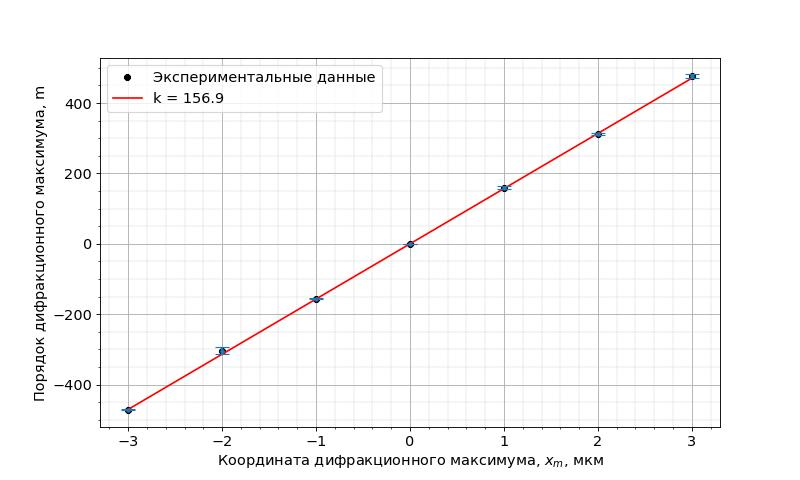
\includegraphics[width=16cm]{image1.jpg}
    \end{center}
    \caption{График зависимости угла дифракции $sin(\varphi_m)$ от длины волны }
    \label{img3}
\end{figure}

    \item По углу наклона графика определим период эшелета, оценили погрешность результата.

\[ |k| = (692.0 \pm 19.3) \text{ }\frac{\text{шт}}{\text{мм}} \]
\[ \Longrightarrow \frac{1}{d} = (692.0 \pm 19.3) \text{ мм} \Longleftrightarrow d = (1.45 \pm 0.1) \text{ мкм.}\]

    \item По формуле рассчитаем угловую дисперсию в рабочем порядке для жёлтого дублета в угловых секундах на ангстрем:

    \[ D=\frac{d\varphi}{d\lambda}, \text{ }d\varphi = (17-12)\cdot60+(4-41)=263 \text{ угл.сек., } d\lambda=5791-5770=21\text{ А}\]
    \[ \Longrightarrow D=\frac{263}{21} = 12.5\text{ }\frac{\text{угл.сек.}}{A}. \]

    \item Ранее оценили экспериментальную разрешающую способность: $R = 3473$. Сравним её с теоретической:

    \[ R^{\text{theory}}=mN, \text{ }m=1\text{ } \Longrightarrow N = 3473. \]

    То есть $3473$ штриха эшелета освещены. При периоде $d=1.45\text{ мкм}$, получаем, что $5.02\text{ мкм}$ освещено. Эшелет освещён частично.

    \item Рассчитаем угол скоса рабочей грани эшелета по формуле:

    \[ 2d\sin{\Omega}=m_p\lambda_p \Leftrightarrow \Omega=\arcsin{\frac{m_p\lambda_p}{2d}} \]
    \[ \Longrightarrow \Omega=\arcsin{\frac{1\cdot5800\cdot10^{-10}}{2\cdot1.7\cdot10^{-3}}} = 9.7\cdot10^{-3} \text{ град.} \]

    \item Используя все экспериментальные данные, рассчитаем угловую дисперсию для жёлтого дублета и косинусы дифракционных углов.

    \begin{table}[h]
        \centering
        \begin{tabular}{|c|c|c|}
        \hline
            \multicolumn{3}{|c|}{$\varphi=45^{\circ}$} \\ \hline
        \hline
        $m_{\text{порядок}}$ & $D, \text{ }\frac{\text{угл.сек.}}{A}$ & $\cos{\varphi_m}$ \\ \hline
            1 & 12.5 & -0.622 \\ \hline
            2 & 25.3 & -0.983 \\ \hline
        \end{tabular}
        \begin{tabular}{|c|c|c|}
        \hline
            \multicolumn{3}{|c|}{$\varphi=60^{\circ}$} \\ \hline
        \hline
        $m_{\text{порядок}}$ & $D, \text{ }\frac{\text{угл.сек.}}{A}$ & $\cos{\varphi_m}$ \\ \hline
            1 & 14.9 & -0.622 \\ \hline
            2 & 25.1 & -0.931 \\ \hline
            3 & 38.4 & -0.999 \\ \hline
        \end{tabular}
        \begin{tabular}{|c|c|c|}
        \hline
            \multicolumn{3}{|c|}{$\varphi=30^{\circ}$} \\ \hline
        \hline
        $m_{\text{порядок}}$ & $D, \text{ }\frac{\text{угл.сек.}}{A}$ & $\cos{\varphi_m}$ \\ \hline
            -1 & 20.9 & -0.726 \\ \hline
            1 & 11.6 & -0.906 \\ \hline
        \end{tabular}
    \caption{Результаты вычислений}
    \label{tab2}
    \end{table}

    \item Построили график зависимости угловой дисперсии $D$ от величины $\frac{m}{\cos{\varphi_m}}$.

    \begin{figure}[h]
        \begin{center}
            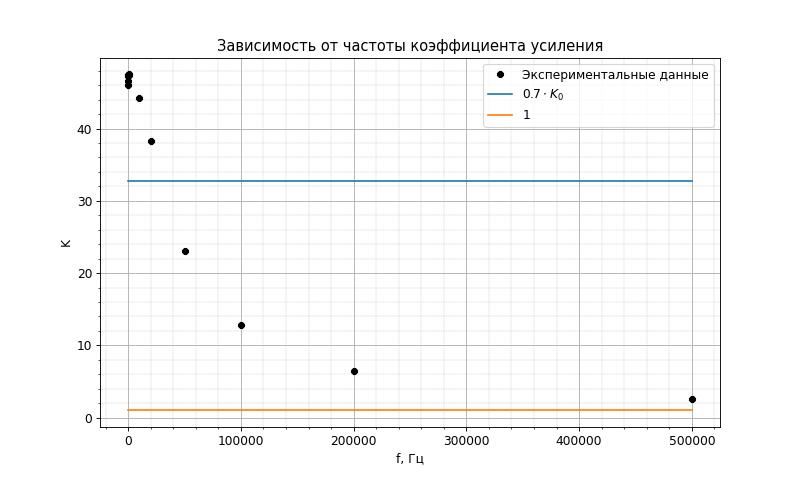
\includegraphics[width=16cm]{image2.jpg}
        \end{center}
        \caption{График зависимости угловой дисперсии от косинусов дифракционных углов при $\psi=45^{\circ}$}
        \label{img4}
    \end{figure}

    \[ |k| = 12.986\text{ }\frac{\text{угл.сек.}}{A} \Longrightarrow d = \frac{3600}{k} = 0.028\text{ мкм}. \]

\newpage

    \begin{figure}[h]
        \begin{center}
            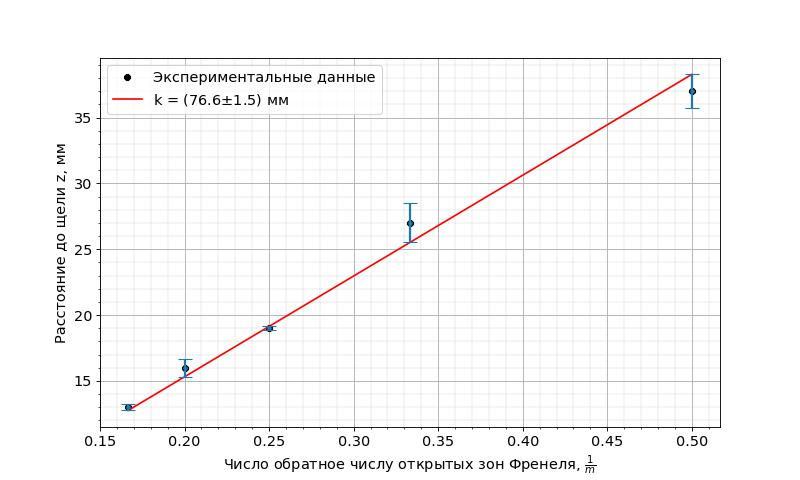
\includegraphics[width=16cm]{image3.jpg}
        \end{center}
        \caption{График зависимости угловой дисперсии от косинусов дифракционных углов при $\psi=60^{\circ}$}
        \label{img5}
    \end{figure}

    \[ |k| = 11.75\text{ }\frac{\text{угл.сек.}}{A} \Longrightarrow d = \frac{3600}{k} = 0.03\text{ мкм}. \]

\newpage

    \begin{figure}[h]
        \begin{center}
            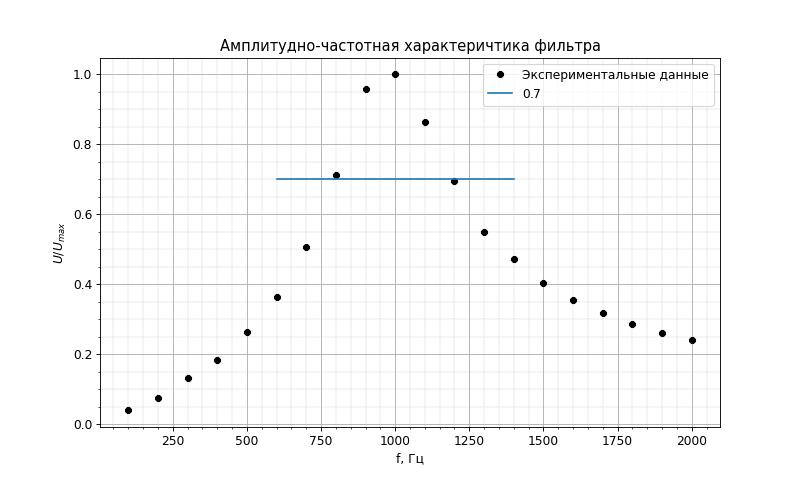
\includegraphics[width=16cm]{image4.jpg}
        \end{center}
        \caption{График зависимости угловой дисперсии от косинусов дифракционных углов при $\psi=30^{\circ}$}
        \label{img6}
    \end{figure}

    \[ |k| = 4.65\text{ }\frac{\text{угл.сек.}}{A} \Longrightarrow d = \frac{3600}{k} = 0.077\text{мкм}. \]

\end{enumerate}

\section{Подведение итогов и выводы}

В ходе лабораторной работы мы изучили принцип действия измерительного прибора-гониометра, а так же спектрального прибора - эшелетта. С помощью эшелетта мы изучили спектр ртутной лампы. 

Так же определили характеристики эшелетта:

\begin{enumerate}
    \item разрешающая способность $R=3473$;
    \item дисперсионная область $D=12.5\text{ }\frac{\text{угл.сек.}}{A}$;
    \item период фазовой решётки $d=(1.7\pm0.1)\text{ мм}$.
\end{enumerate}

В последнем пункте мы пытались измерить период фазовой решётки другим способом, предложенным в работе. К сожалению, результаты не совпали с вычисленным ранее, а погрешность определить невозможно, поскольку график строился по двум точкам. Тем не менее, другие результаты нашей работы хорошо соотносятся с теоретическими, что говорит о точности измерений с помощью гониометра.

    
    

\end{document}
